\section{Work Breakdowns and Resources}

\noindent One of the main purposes of this document is to define the tracking trigger R\&D project and organize the efforts. In this section, we will describe possible work breakdowns and work packages for the Vertical Slice System Demonstration. The main work involved can be roughly divided into seven areas, and is shown in Figure z below. These seven areas can be future organized as seven Work Packages (see Figure z1)�.

\begin{figure}[ht!]
\centering
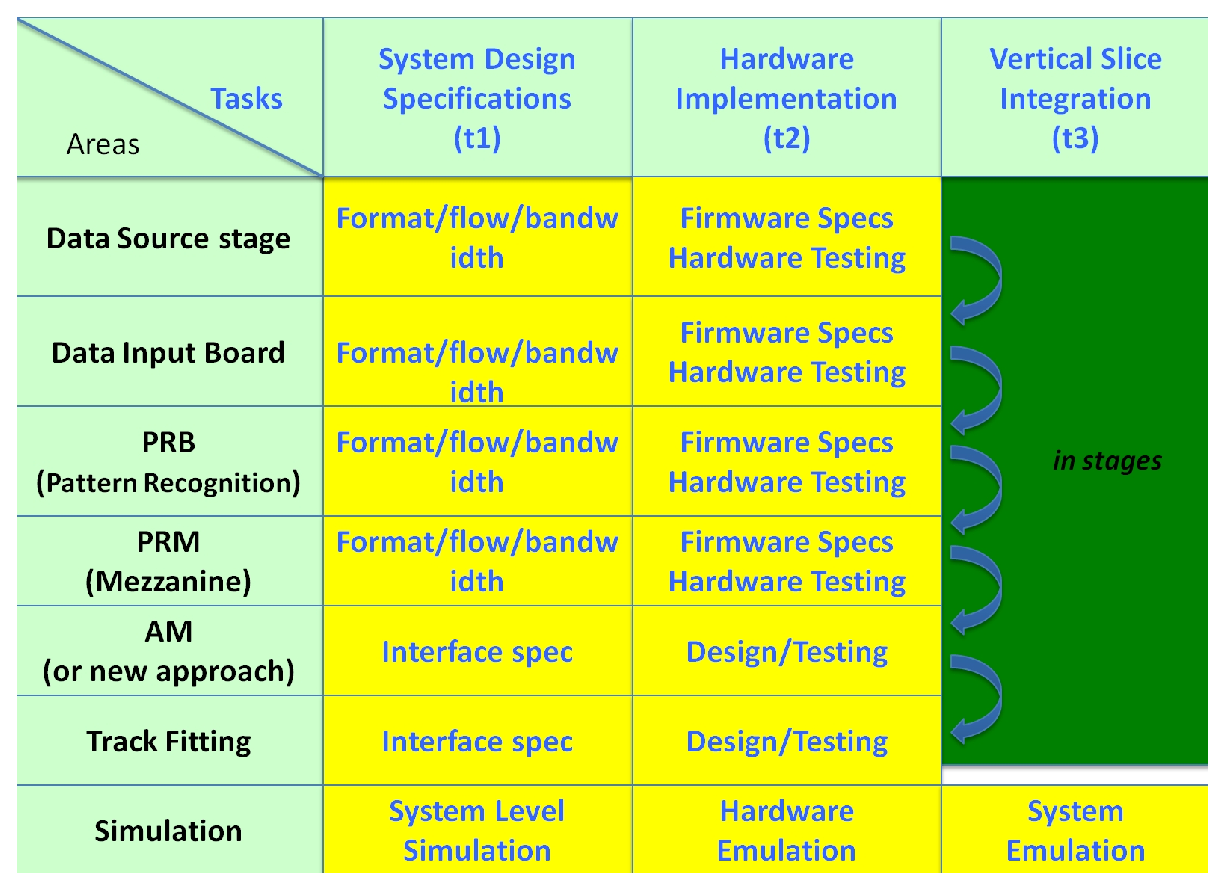
\includegraphics[width=0.7\columnwidth]{Plots/WP.eps}
\caption{Work packages}
\label{fig:WP}
\end{figure}

\begin{figure}[ht!]
\centering
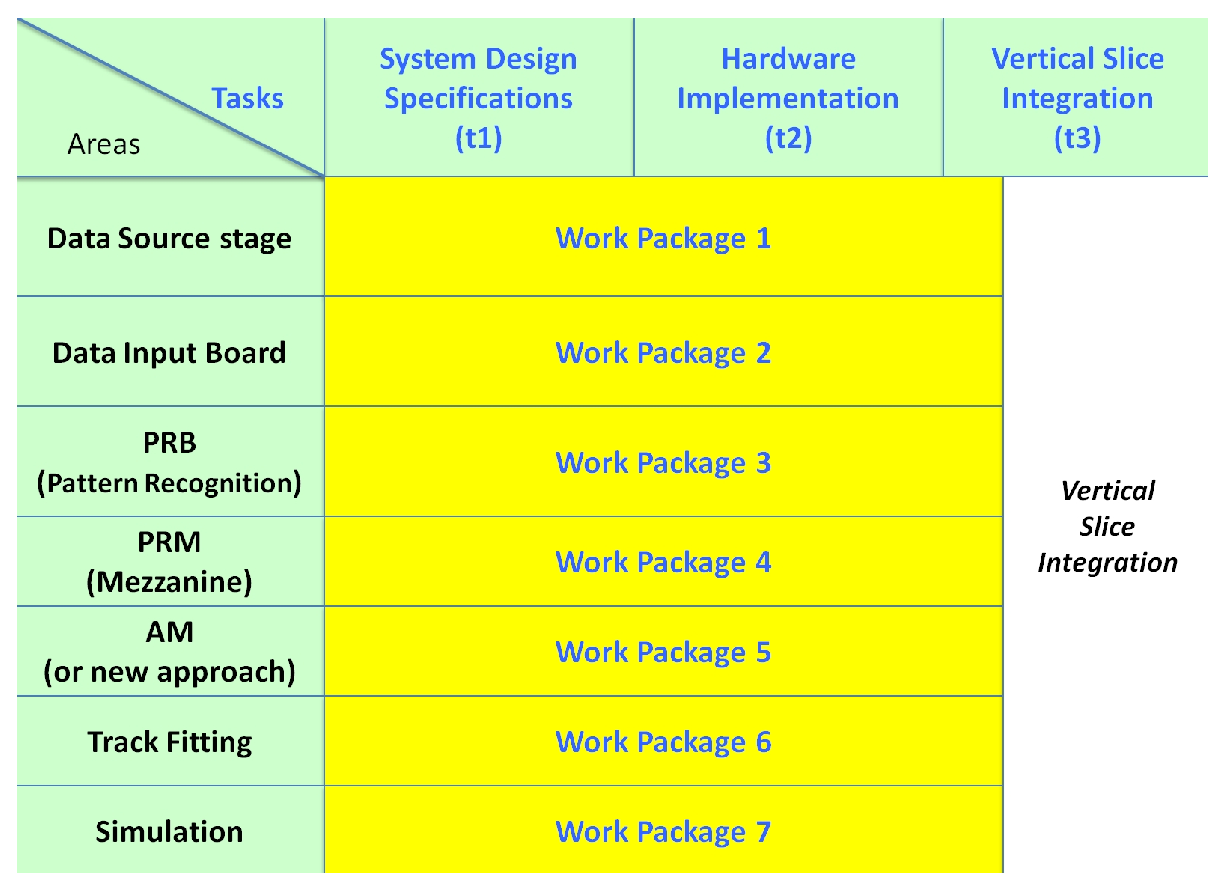
\includegraphics[width=0.7\columnwidth]{Plots/WP2.eps}
\caption{Work packages}
\label{fig:WP2}
\end{figure}

\begin{figure}[ht!]
\centering
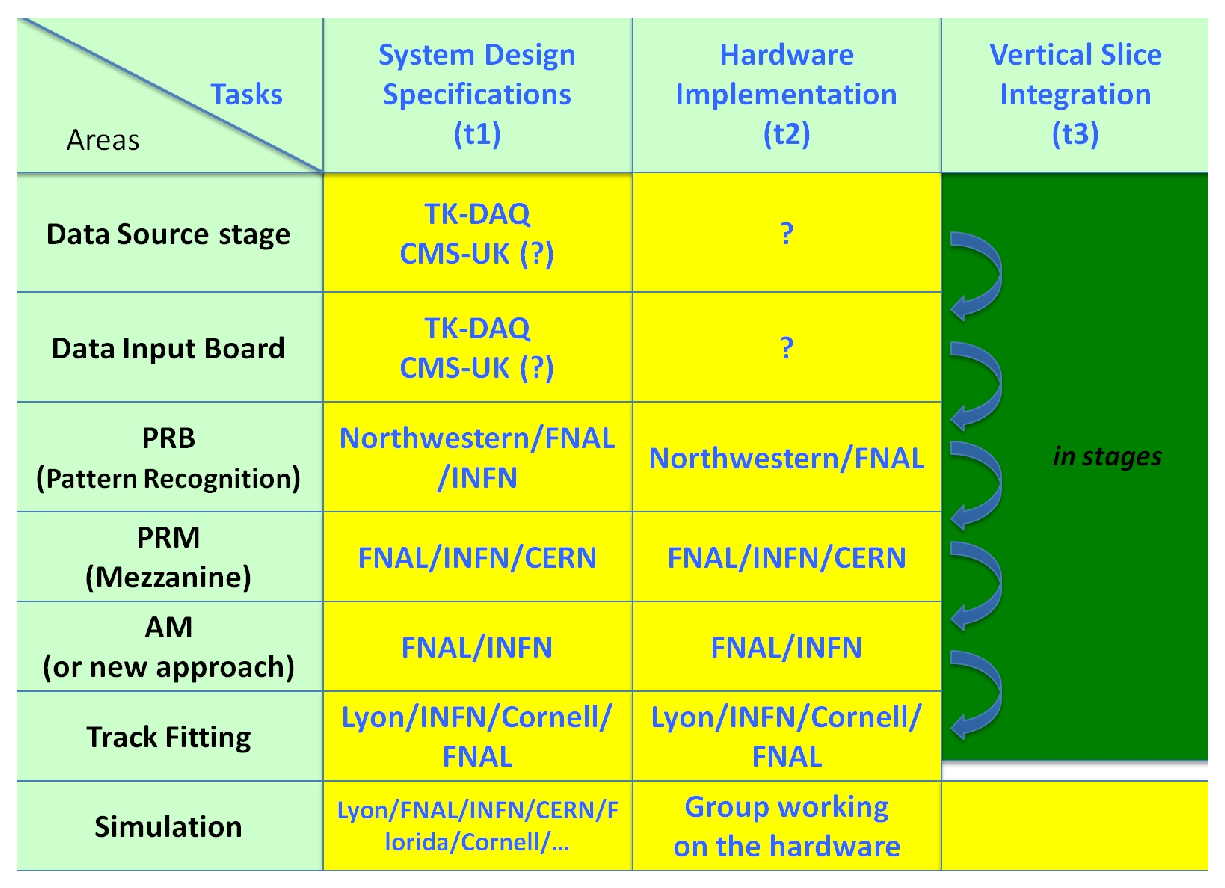
\includegraphics[width=0.7\columnwidth]{Plots/Sharing.eps}
\caption{Current involvments}
\label{fig:Sharing}
\end{figure}


\clearpage
